%LTeX: language=en-CA
% First Draft for ECON807 Policy Project
% Daniel Sánchez Pazmiño
% ECON807 Spring 2023

% Requires the data-preparation.R to run.

\documentclass[11pt,a4paper]{article}\usepackage[]{graphicx}\usepackage[]{xcolor}
% maxwidth is the original width if it is less than linewidth
% otherwise use linewidth (to make sure the graphics do not exceed the margin)
\makeatletter
\def\maxwidth{ %
  \ifdim\Gin@nat@width>\linewidth
    \linewidth
  \else
    \Gin@nat@width
  \fi
}
\makeatother

\definecolor{fgcolor}{rgb}{0.345, 0.345, 0.345}
\newcommand{\hlnum}[1]{\textcolor[rgb]{0.686,0.059,0.569}{#1}}%
\newcommand{\hlstr}[1]{\textcolor[rgb]{0.192,0.494,0.8}{#1}}%
\newcommand{\hlcom}[1]{\textcolor[rgb]{0.678,0.584,0.686}{\textit{#1}}}%
\newcommand{\hlopt}[1]{\textcolor[rgb]{0,0,0}{#1}}%
\newcommand{\hlstd}[1]{\textcolor[rgb]{0.345,0.345,0.345}{#1}}%
\newcommand{\hlkwa}[1]{\textcolor[rgb]{0.161,0.373,0.58}{\textbf{#1}}}%
\newcommand{\hlkwb}[1]{\textcolor[rgb]{0.69,0.353,0.396}{#1}}%
\newcommand{\hlkwc}[1]{\textcolor[rgb]{0.333,0.667,0.333}{#1}}%
\newcommand{\hlkwd}[1]{\textcolor[rgb]{0.737,0.353,0.396}{\textbf{#1}}}%
\let\hlipl\hlkwb

\usepackage{framed}
\makeatletter
\newenvironment{kframe}{%
 \def\at@end@of@kframe{}%
 \ifinner\ifhmode%
  \def\at@end@of@kframe{\end{minipage}}%
  \begin{minipage}{\columnwidth}%
 \fi\fi%
 \def\FrameCommand##1{\hskip\@totalleftmargin \hskip-\fboxsep
 \colorbox{shadecolor}{##1}\hskip-\fboxsep
     % There is no \\@totalrightmargin, so:
     \hskip-\linewidth \hskip-\@totalleftmargin \hskip\columnwidth}%
 \MakeFramed {\advance\hsize-\width
   \@totalleftmargin\z@ \linewidth\hsize
   \@setminipage}}%
 {\par\unskip\endMakeFramed%
 \at@end@of@kframe}
\makeatother

\definecolor{shadecolor}{rgb}{.97, .97, .97}
\definecolor{messagecolor}{rgb}{0, 0, 0}
\definecolor{warningcolor}{rgb}{1, 0, 1}
\definecolor{errorcolor}{rgb}{1, 0, 0}
\newenvironment{knitrout}{}{} % an empty environment to be redefined in TeX

\usepackage{alltt}

% ========================================= Preamble ========================================= %

% ---- Document Parameters ---- %

\title{The influence of entry regulation on formal employment \\[1em] 
\large{ECON 807 Macroeconomic Theory \& Policy Policy Project Final Draft}\footnote{
Length: 12 pages, not including references or appendices. \\
This file has been uploaded with a \texttt{.rar} file including the R project which replicates the environment upon which this paper was written. Also, review the paper's \href{https://github.com/dsanchezp18/econ807-policy-project}{GitHub repository} to quickly glance at the data preparation or the model estimation and data visualization in a \texttt{.Rnw} file (R Sweave/Knitr). The paper's source code is in the \texttt{final} folder in the repository.}}
\author{Daniel Sánchez Pazmiño}
\date{April 2023}

% ---- Load LaTeX packages ---- %

% Format

\usepackage[margin = 1in]{geometry}

% Tables 

\usepackage{booktabs}
\usepackage{siunitx}
\newcolumntype{d}{S[
    input-open-uncertainty=,
    input-close-uncertainty=,
    parse-numbers = false,
    table-align-text-pre=false,
    table-align-text-post=false
 ]}

% Referencing

\usepackage[backend = biber, style = apa, citestyle = apa]{biblatex}
  \addbibresource{refs.bib}

% Misc
\usepackage{hyperref}

% ---- Preamble Chunks ----- %



% ----- Document ----- % 
\IfFileExists{upquote.sty}{\usepackage{upquote}}{}
\begin{document}

\maketitle

\begin{abstract}

Informal labour markets are very prevalent in Latin America, where often political blockage difficults passing legislation which can address these issues directly. Alternative policies may be taken into account to help tackle the issue of informal work. In this paper, I explore the effect of an entry cost deregulation reform which happened in Ecuador in May 2020. An event-study approach is taken for the empirical analysis with a theoretical framework proposed by \textcite{Branstetter.2014}. While the empirical analysis shows mixed results, there is significant evidence which supports the fit of the theoretical with the data. In this sense, it is possible that a reduction in fixed entry costs for firms can create employment, but such reduction should be large enough to have a statistically significant effect.
\end{abstract}

\section{Introduction}

It is well known that informal work -legal but informal economic activities which occur outside the government's regulatory capability \parencite{Sassen.1994}- can hinder economic development through several channels. Informal firms reduce the amount of taxes that can be collected and these businesses tend to remain relatively smaller and less efficient. Informality is also related to bigger gender gaps, higher inequality, lower education and other negative outcomes \parencite{Delechat2020}. Additionally, informal sector workers often lack access to social security and other employment benefits and tend to earn lower wages. The informal economy has been characterized with poorly defined work spaces, unsafe and unsanitary working conditions, long working hours and a lack of access to markets, financial services, training, and technology \parencite{IloND}. 

While less present in the developed world, informality is very prevalent in developing countries, where it represents a third of low and middle-income countries' economic activity \parencite{Delechat2020}. The work of \textcite{Soto.2002} has motivated much research about informality in Latin America, being one of the regions with the most prevalent levels of informality, as it often is the only option for several workers on the lower end of the wealth distribution \parencite{Oviedo.2009}. At the macroeconomic level, informality could be regarded at the institutional level, which has been shown to be a significant factor for growth \parencite{Acemoglu.2001, RafaelLaPorta.1997, Glaeser.2004}. Further, its effect on inequality and its potential as a channel for propagation of monetary and fiscal policy \parencite{Alberola.2020} make informality a significant macroeconomic determinant of development.

The desire for the formalization of the economy is thus well understood, especially considering that the COVID-19 pandemic has increased informality worldwide \parencite{ILO.2022}. However, the policy angle is subtle, given that the causes and consequences of informality are difficult to document and understand. Some approaches have focused on the role of governments in providing incentives for formalization. Designing tax systems that minimize distortions in the market \parencite{Bardey.2019} as well as reducing the costs of formalization by reducing firm entry regulation are some of this approach's implementations. \textcite{MauricioPrado.2011} proposes that firms which are less productive endogenously choose to operate informally due to entry costs and taxation. Thus, reducing entry costs can directly affect formalization of businesses, which may impact formal employment.

\begin{figure}[h]
\caption{Active formal businesses and job contracts registered under Social Security in Ecuador}
\label{fig:fig}
\begin{knitrout}
\definecolor{shadecolor}{rgb}{0.969, 0.969, 0.969}\color{fgcolor}
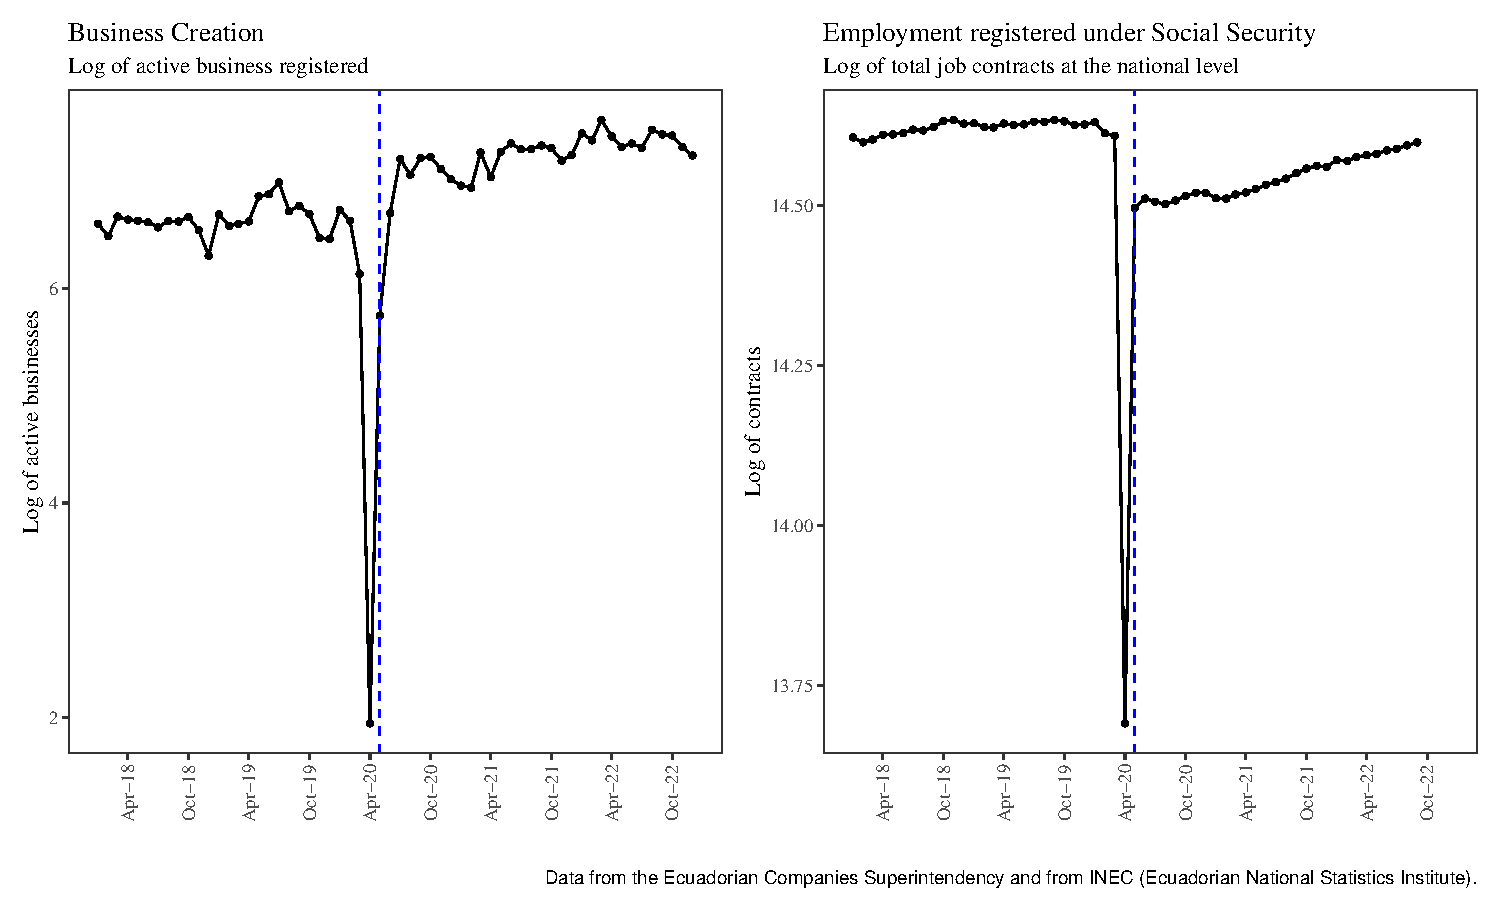
\includegraphics[width=\maxwidth]{figure/figure-1-1} 
\end{knitrout}
\end{figure}

In this paper, I investigate the relationship between entry regulation and labour market formalization by exploiting an exogenous shock on entry regulation in Ecuador. By using administrative data from various Ecuadorian public institutions and a comprehensive event study or interrupted time series empirical framework, I exploit variation in formal employment across time at the province level in Ecuador before and after the reform. The policy change was enacted in May 2020 and allowed for the creation of a new legal form of business, the \textit{Sociedad de Acciones Simplificada}\footnote{In English, \textit{Simplified Shares Society.}} (SAS). The reform sought to reduce monetary and time costs relative to other legal figures in the firm creation process, and has proven to be effective in doing so and fostering business creation \parencite{CaminoMogro.2022}. Figure \ref{fig:fig} displays all active businesses before and after the policy change as well as the amount of job contracts registered under Social Security in Ecuador, showing how employment and business creation tend to move together.

I base my empirical analysis on a theoretical framework informed by the work of \textcite{Branstetter.2014}. In a simple model of entrepreneurship it is predicted that reduced entry costs will increase firm entry and employment, however, all impacts are \textit{at the margin}: new firms will be generally smaller, less productive and less likely to hire large amounts of new workers. While the results from the empirical analysis show a small positive effect of the reform on employment, the effect is not robust across different specifications. Further, event study specifications suggest that due to the timing of the policy, the immediate effects of the policy might be due to catch-up effects from the pandemic rather than due to the reform itself. These results suggest that the true causal effect of the policy on employment may be too small to identify with this empirical strategy. However, an important and robust finding is that the model seems to support the Ecuadorian data, as it did with the empirical validations in Portugal \parencite{Branstetter.2014} and Mexico \parencite{Kaplan.2011}, who find small positive effects of entry cost deregulation. However, the possibility of a null effect of the reform in Ecuador might be explained by the lack of coordination between entry and labour market regulation, as well as the weaknesses of the present empirical design.

I contribute to the very reduced stream of the literature which analyses the impact of entry regulations on employment, considering the existence of informal and formal sectors. Further, the use of administrative instead of survey data enhances the possibilities of extracting insight which is valid at any level of aggregation. No other research links these types of policies to the creation of formal employment, given that these policies are more geared towards fostering entrepreneurship. However, given that \textcite{Branstetter.2014} identifies marginal firms as smaller, which are more likely to be informal \parencite{ElianeElBadaoui.2010}, entry cost regulation may be an important policy tool for tackling informality, especially when labour market reform is politically blocked, as is the case of Ecuador. 

\section{Literature Review}

The literature on informality and entry cost regulation is extensive, but few papers explore the relationship between the two. The theory points to informality being an endogenous decision, where firms with low productivity often prefer to remain informal, the size of the firm often being an important determinant of this decision \parencite{Delechat2020, MauricioPrado.2011, ElianeElBadaoui.2010}. This endogeneity makes informality difficult to investigate empirically: many informal workers are not officially registered and may not report their activities accurately \textcite{Oviedo.2009}. In the macroeconomic context, it has been shown that informality lowers TFP, increases output volatility and may produce significant input misallocation. Further, informal jobs have been found to respond heavily to changes in formal employment \parencite{Leyva.2020}.

Research on Ecuador is limited and has focused on the effect of exogenous shocks on measurements of informality, notably measuring the effects of an earthquake in 2016 \parencite{Mendoza.2020} and the labour market impact of Venezuelan migration \parencite{Olivieri.2022}, both finding positive effects on informality. It is found that poverty and informality are jointly determined, where informal workers often come from low education and low income backgrounds. Further, the informal labour market is mainly supply-led but it is so heterogenously: low-skilled workers often have no choice to work informally, while better educated workers sometimes choose to operate informally \parencite{Canelas.2019}. On the firm side, it is determined that the endogenous choice of sector is also present in Ecuador \parencite{Medvedev.2016}. Ecuador also documents a formal sector wage premium \textcite{MacIsaac.1997}, which, according to \textcite{ElianeElBadaoui.2010}, responds to a firm size wage premium due to the endogenous choice of the firm to operate in the informal sector. 

Estimating the size and nature of the informal economy and to assess the impact of policies aimed at reducing informality is difficult, however, one common idea that has come up as a policy angle is reducing distortions for businesses by simplifying entry regulation. These types of policies have been implemented across Latin America as well as in Europe, which have had positive results \parencite{Oviedo.2009}. However, research has been focused on the policy's effectiveness at creating formal businesses, not measuring their labour market impact. \textcite{Branstetter.2014} develop a simple entrepreneurship model and validate it with a reduction of entry costs in Portugal, finding the reform significantly impacted business creation but mostly for marginal firms. These marginal firms were typically small, owned by relatively poorly educated entrepreneurs, and operating in low-technology sectors and less likely to survive after two years. Employment effects of the reform were positive but small, as was the case of a Mexican deregulation of entry by \textcite{Kaplan.2011}. Further, \textcite{Bertrand.2002} find that both product market and entry regulation were sources of employment growth in France in the 1970s, focusing on the retail sector in France. Further, a macroeconomic study of product and labour market regulation, modelled as higher entry costs, links higher levels of regulations to lower employment \parencite{Blanchard.2003}. However, none of these papers acknowledge the existence of formal and informal sectors.

\section{Theoretical Framework}

I use the theoretical model of entrepreneurship proposed by \textcite{Branstetter.2014} to guide my empirical analysis. In this model, individuals with different entrepreneurial ability endowments $\theta$ are drawn from a continuous probability distribution. Individuals have the possibility to (a) work in the labour market for a wage rate $w$, (b) become an entrepreneur or (c) consume leisure. The payoff to being an entrepreneur, $\pi$ is

\begin{equation}
  h(\theta) + \eta
\end{equation}

where $h$ is a function of the agent's entrepreneurial ability and $\eta$ is an idiosyncratic term, also drawn from a probability distribution and unknown to the entrepreneur before starting their entrepreneurship operation. By defining $h$ as Cobb-Douglas, considering only labour $L$ as a production input and introducing two periods, it is possible to define two profit functions, where the difference between the two is that a fixed cost $F$ is included in $\pi_t$ for $t = 1$ but not for $t=2$ and $\eta$ is revealed to the agent in $t=2$. 

The value for operation as an entrepreneur depends on the level of entrepreneurial ability relative to the market wage rate $w$ as well as on fixed costs $F$. The model predicts that a decrease on $F$ increases the value of entrepreneurship, allowing for more business entry. Further, the level of employment depends on the level of entrepreneurship, and each entrepreneur's labour demand will depend once again on their endowment $\theta$ relative to $w$. Any decrease in $F$ will increase overall employment, considering that there will be more entrepreneurs. However, since reductions in $F$ will work \textit{at the margin}, all extra entrepreneurs will have relatively low $\theta$ and thus smaller labour demand.

This model does not consider the level of capital $K$ and liquidity constraints, and assumes that all workers are hired formally. By observing formal employment fluctuations, it is possible to apply this model to the empirical analysis. However, the model is not able to explain changes in informal employment per se, only changes in formal employment. The extent to which changes in formal employment relate to informal employment is dependent on the ability to observe the pre-policy status of workers hired after the policy change, which is out of the scope of this paper.

\section{Institutional Background}

Ecuador is a middle income country located in upper South America next to Colombia and Peru. The country is comprised of twenty-four provinces across four regions and all provinces encompass a central unified republic. After its full dollarization in 2000, the country saw an economic surge between 2007-2014 as a result of high oil prices and a relatively indebted government \parencite{Weisbrot.2017}. However, after a sharp decline in oil prices and the COVID-19 pandemic, the country seems to be unable to return to its pre-pandemic levels, with employment indicators at an all-time low. 

However, informality and underemployment\footnote{The Ecuadorian National Institute of Statistics considers ``adequate employment'' as people with a job who earn labour income equal to or greater than the minimum wage on an hourly basis. In this sense, underemployment in this paper is considered as any employment which does not comply with this condition.} in this labour market have been shown to be historically high \parencite{Meneses.2021, Chavez.2012, Mendoza.2020}. Further, minimum wage increases in Ecuador (which have been frequent and substantial) have had no effect on employment levels due to high-level of non-compliance and informality in the labour market \parencite{Canelas.2014}. Further, Ecuador has been shown to have one of the most cumbersome labour market legislations in the region \parencite{MacIsaac.1997}, whose effect is attenuated by smaller base earnings over which benefits are paid.

Not only the labour market is highly regulated in the country: the business environment in Ecuador is cumbersome, including several regulatory costs which could create inefficiencies. Ecuador constantly ranks very low in terms of property rights, judicial transparency and economic freedom, which may respond to a flawed and corrupt judiciary, characterized by inefficiency and difficulty to start a business \textcite{Euromonitor.2022}. Further, an unstable economic and political environment after the election of conservative businessman Guillermo Lasso not long after a decade-long leftist regime has taken a toll on the government's financing capabilities. The political instability has also made the deregulation of labour markets difficult: only one set of market-friendly policies set forth by the new president have been passed, the labour market reform being immediately rejected by a strong opposing majority in Congress. Thus, other types of reforms which indirectly target the labour market would be welcome. 

There are several legal figures under which a firm may operate on the Ecuadorian economy. If the firm is fully informal, we may not observe any kind of registry of their economic activity. Most of underemployment comes from this kind of firms, where household members become informal entrepreneurs by selling services or goods informally. However, \textit{partially formal} employment is quite prevalent, and in this scheme the figure of a ``tax contributor'' becomes relevant. There are differentiated tax figures for entrepreneurs in Ecuador: most fall under a ``microbusiness'' which need not establish a formal company but merely have a \textit{registro único de contribuyente}\footnote{Unique contributor registration} (RUC), which is a tax identificator number which allows those registered to issue invoices and pay value-added tax. Having a RUC is relatively low cost compared to establishing a company, yet there is a revenue limit: if any firm exceeds such limit, it must pay more taxes or constitute a legal company figure. A lot of informal work comes from these types of legal figures, which creates the need to control for tax contributor changes across provinces and time, which is possible due to SRI data.

The SAS reform, enacted in May 2020, allowed a new type of legal business to exist, which also exists in other countries in the region. This type of business is known to be much less burdensome than other types of companies like anonymous societies or limited liability companies. A SAS business can be created with lower monetary and time costs (notarization, registering, etc.) as well as with lower amounts of capital contributions. The SAS company would allow an informal firm working under a RUC scheme to easily transition to a formal company. It is sensible to believe that the reform was unexpected and exogenous since, while the law that allowed for this reform came into force in early 2020, the law did not specifically plan for the creation of this type of business, only allowed for its creation under corporate law. Further, \textcite{CaminoMogro.2022} find causal evidence that this reform was effective in formalizing/creating businesses and in reducing time and money entry costs. However, the effects of the policy in the labour market have not been studied so far. 

\section{Methodology}
\subsection{Data}
I construct a province-month panel dataset of the country with variables stemming from various government sources. The variables of interest are the natural logarithms of (1) total job contracts registered with Social Security and (2) total job contracts registered under the unique Ecuadorian Labour System (SUT, for its initials in Spanish). The latter is a more reduced measure of formal employment, but it should move with Social Security job contracts.

Table \ref{tab:sources} in the Appendix defines all variables used in the paper along with their source. Any kind of job contract which is registered in Social Security is thought to be formal, as Social Security formalization implies that all employment benefits mandated by the Ecuadorian Labour Code are being met by the employer and the government. The same applies for formal job contracts registered under SUT. 
\begin{table}[h]
\caption{Mean values by year}
\label{tab:descrip}
\centering

\begin{tabular}[t]{lrrrrr}
\toprule
  & 2018 & 2019 & 2020 & 2021 & 2022\\
\midrule
Formal jobs & \num{10.24} & \num{10.23} & \num{10.16} & \num{10.08} & \num{10.14}\\
Formal jobs (SUT) &  &  & \num{5.24} & \num{5.71} & \num{6.39}\\
Active businesses & \num{2.24} & \num{2.52} & \num{2.42} & \num{2.84} & \num{3.05}\\
Remote workers & \num{0.93} & \num{1.37} & \num{3.15} & \num{2.37} & \num{1.79}\\
Registered tax contributors & \num{10.54} & \num{10.61} & \num{10.69} & \num{10.76} & \num{10.87}\\
Reported sales & \num{18.80} & \num{18.81} & \num{18.71} & \num{18.81} & \num{18.96}\\
Total COVID-19 cases &  &  & \num{6.41} & \num{6.47} & \num{6.43}\\
Total COVID-19 deaths &  &  & \num{2.97} & \num{2.64} & \num{1.96}\\
Thefts & \num{4.57} & \num{4.59} & \num{4.24} & \num{4.38} & \num{4.57}\\
Homicides & \num{1.10} & \num{1.18} & \num{1.25} & \num{1.46} & \num{1.91}\\
Transit Accidents & \num{1.04} & \num{1.10} & \num{1.01} & \num{0.92} & \num{1.14}\\
Inscriptions & \num{6.36} & \num{6.51} & \num{5.83} & \num{6.08} & \num{6.29}\\
Suspensions & \num{6.48} & \num{6.53} & \num{6.02} & \num{6.38} & \num{6.39}\\
Total mobility &  &  & \num{-19.42} & \num{9.20} & \num{37.08}\\
\bottomrule
\end{tabular}


\vspace{0.3cm}
All variables in natural log form. See Appendix A for data sources.
\end{table}
\subsection{Empirical Strategy}

To identify the causal effect of the SAS reform on formal job creation, I take an event-study approach with a regression framework (interrupted time series) in the lines of \textcite{Taljaard.2014}. Given that Ecuador is a unified republic, I do not observe variation in treatment across the cross-section. I take pre-event data as my control group, and use the event study framework to evaluate this assumption. Two approaches are implemented: segmented regressions using an interaction term between a time trend and a ``treatment'' dummy after the date of the policy change, and event study specifications using month-year dummies across the study's horizon. The segmented regressions take the following general form:

\begin{equation}
\label{eqn:seg}
\ln(L)_{it} = \phi_i + \beta_1 time + \delta_0 treatment_{i} + \delta_1(time \cdot treatment_{i}) + \mathbf{x}_{it}'\gamma + u_{it}
\end{equation}

where $L$ is the number of formal job contracts, observed for provinces $i = 1, 2, ..., N$ and months $t = 1,2 ..., T$. In this paper, I measure $L$ using two different indicators from the Ecuadorian government; main results are reached with Social Security contracts and Appendix \ref{sec:appc} displays results using SUT job contracts. $\phi_i$ are a set of province fixed effects, where Pichincha (where the capital is located) is the reference province. $u_{it}$ is an error term, considering unobserved variables within provinces which change across time. $t$ is a time trend variable, centered around May 2020, for which I consider alternative polynomials. The treatment dummy equals unity for all provinces observed in May 2020 or after. $\mathbf{x}_{it}$ is a vector of province-specific time-varying covariates used as controls which are thought to potentially influence $L$ and did not remain smooth across the date of the policy change. These are all used in their natural logarithm form, except for the Google Mobility data, which is presented as percent deviations from the baseline (January 2020). In some cases, to account for an autoregressive process, I account with the a lag of the explained variable, $\ln(L)_{it-1}$.

Ultimately, I am interested in the $\hat{\delta}_1 $ parameter, which measures the change in the time trend of $\ln(L)_{it}$ at the time of the policy change. This parameter can be interpreted as the causal effect of the SAS reform on formal job creation if there are no confounding effects, that is, unobserved factors left in the error term $u_{it}$ which changed in $t = 0$ and affect formal employment.

For the event study specifications, I consider the following general form:

\begin{equation}
\label{eqn:event}
\ln(L)_{it} = \phi_i + \tau_t + \mathbf{x}_{it}'\gamma + u_{it}
\end{equation}

where the new $\tau_t$ are a set of period fixed effects. The sign of the fixed effects after May 2020 will be ilustrative of the effect of the policy change on the outcome. Further, these event study specifications allow me to look at the pre-policy change trend for $\ln(L)_{it}$, thus being able to test the assumption that all pre-treatment effects are null \parencite{HuntingtonKlein.2021}. For all specifications, I present clustered standard errors at the province and month level, but also consider autocorrelation-robust standard errors (HAC). 

\section{Results}
Table \ref{tab:regseg} displays OLS estimation results for the empirical model specified in Equation \ref{eqn:seg} and Table \ref{app:seg} in Appendix B presents the same results but with HAC standard errors. Model 1 below estimates a naive segmented regression model considering only the treatment dummy interacted with the time trend. The interaction between the time trend and the treatment dummy is not statistically significant. The negative and statistically significant coefficient on the treatment dummy means that, as time passed, there seemed to be a negative trend after the date of the policy. Model 2 estimates the same naive model but now considering province fixed effects, which control for all province-specific factors which affect formal employment yet stay constant through time. In this case, including fixed effects renders the interaction term positive and significant. Potentially, the $\hat{\delta_1}$ coefficient in Model 1 is biased toward zero as it is possible that some provinces with less economic activity suffered from staggered pandemic effects after the policy change. If other provinces saw a positive effect, it would mean that the average effect on the naive regression would be biased toward zero.
\begin{table}[htbp!]
\caption{Segmented Regressions}
\label{tab:regseg}

\begin{tabular}[t]{lcccccc}
\toprule
  & (1) & (2) & (3) & (4) & (5) & (6)\\
\midrule
Time & \num{0.003}* & \num{0.000} & \num{0.001} & \num{-0.004}*** & \num{0.001} & \num{0.001}\\
 & (\num{0.002}) & (\num{0.001}) & (\num{0.001}) & (\num{0.001}) & (\num{0.001}) & (\num{0.001})\\
Time (quadratic) &  &  &  & \num{0.000}*** & \num{0.000} & \num{0.012}***\\
 &  &  &  & (\num{0.000}) & (\num{0.000}) & \vphantom{1} (\num{0.002})\\
Treatment & \num{-0.237}*** & \num{-0.152}*** & \num{-0.120}*** & \num{-0.074}*** & \num{-0.007} & \num{0.031}***\\
 & (\num{0.030}) & (\num{0.026}) & (\num{0.014}) & (\num{0.017}) & (\num{0.009}) & (\num{0.009})\\
Interaction & \num{0.001} & \num{0.003}*** & \num{0.001} &  &  & \\
 & (\num{0.002}) & (\num{0.001}) & (\num{0.001}) &  &  & \\
Interaction (quadratic) &  &  &  & \num{0.000}*** & \num{0.000} & \num{-0.012}***\\
 &  &  &  & (\num{0.000}) & (\num{0.000}) & (\num{0.002})\\
WFH workers &  &  & \num{0.001} & \num{0.001} & \num{0.000} & \num{0.000}\\
 &  &  & (\num{0.002}) & (\num{0.002}) & (\num{0.001}) & (\num{0.001})\\
Thefts &  &  & \num{0.020} & \num{0.012} & \num{0.008} & \num{-0.001}\\
 &  &  & (\num{0.017}) & (\num{0.017}) & (\num{0.007}) & (\num{0.008})\\
Homicides &  &  & \num{0.003} & \num{0.002} & \num{0.001}* & \num{0.001}\\
 &  &  & (\num{0.004}) & (\num{0.004}) & (\num{0.001}) & (\num{0.002})\\
Tax contributors &  &  & \num{-0.081} & \num{-0.094} & \num{-0.041} & \num{-0.095}*\\
 &  &  & (\num{0.058}) & (\num{0.068}) & (\num{0.035}) & (\num{0.054})\\
Sales &  &  & \num{0.039}** & \num{0.033}** & \num{0.006} & \num{0.000}\\
 &  &  & (\num{0.017}) & (\num{0.013}) & (\num{0.004}) & (\num{0.005})\\
Transit Accidents &  &  & \num{0.003} & \num{0.002} & \num{-0.001} & \num{-0.002}\\
 &  &  & (\num{0.002}) & (\num{0.002}) & (\num{0.001}) & (\num{0.002})\\
Businesses &  &  &  &  & \num{0.006}** & \num{0.007}\\
 &  &  &  &  & (\num{0.003}) & (\num{0.004})\\
Lag of jobs &  &  &  &  & \num{0.942}*** & \num{0.870}***\\
 &  &  &  &  & (\num{0.031}) & (\num{0.065})\\
COVID-19 cases &  &  &  &  &  & \num{0.000}\\
 &  &  &  &  &  & \vphantom{1} (\num{0.002})\\
COVID-19 deaths &  &  &  &  &  & \num{-0.001}\\
 &  &  &  &  &  & (\num{0.002})\\
Inscriptions &  &  &  &  & \num{0.007}*** & \num{-0.004}\\
 &  &  &  &  & (\num{0.002}) & \vphantom{1} (\num{0.003})\\
Suspensions &  &  &  &  & \num{0.002} & \num{0.004}\\
 &  &  &  &  & (\num{0.002}) & (\num{0.003})\\
Mobility &  &  &  &  &  & \num{0.000}\\
 &  &  &  &  &  & (\num{0.000})\\
\midrule
AIC & \num{4708.41} & \num{-3771.83} & \num{-1855.13} & \num{-1909.57} & \num{-2732.13} & \num{-1380.83}\\
BIC & \num{4729.17} & \num{-3631.68} & \num{-1736.68} & \num{-1787.04} & \num{-2593.33} & \num{-1263.06}\\
Province FE &  & X & X & X & X & X\\
\bottomrule
\end{tabular}


\vspace{0.3cm}
\textbf{Note:} Segmented regression models across multiple specifications. Standard errors are clustered at the month-year and province level.\\
$ *p < 0.1, **p < 0.05, ***p < 0.01.$
\end{table}
\begin{figure}[htbp!]
\caption{Event study plots}
\label{fig:event}
\begin{knitrout}
\definecolor{shadecolor}{rgb}{0.969, 0.969, 0.969}\color{fgcolor}
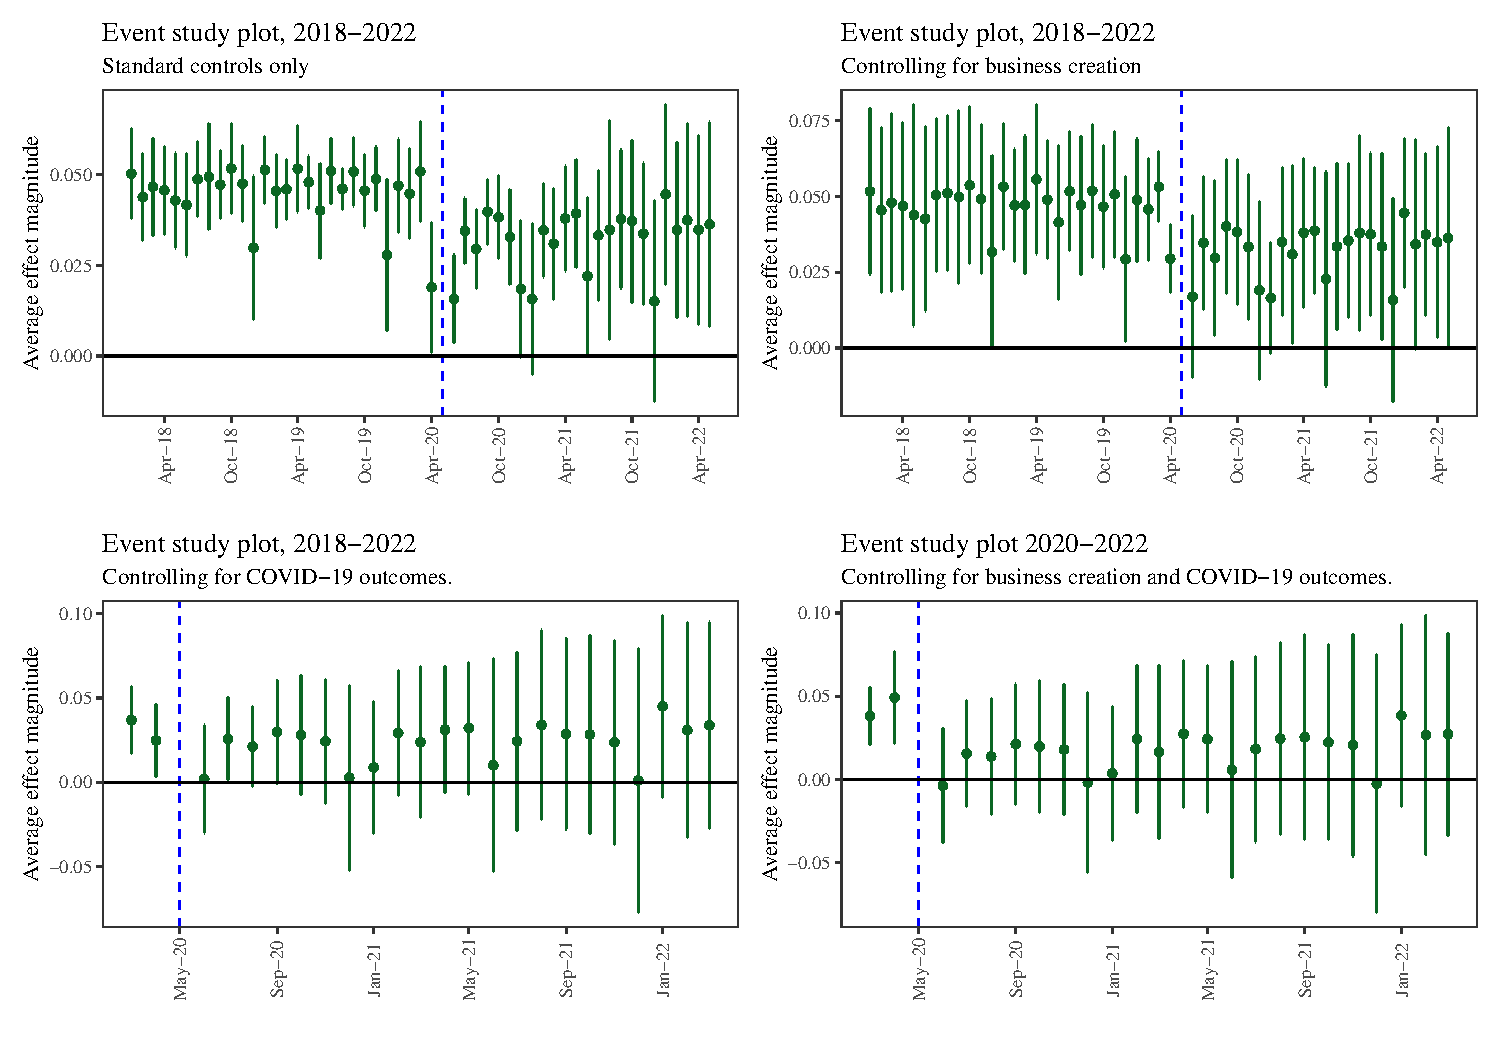
\includegraphics[width=\maxwidth]{figure/event-study-1} 
\end{knitrout}
\textbf{Notes:} Event study plots where the coefficients of period dummies are plotted against time. The reference level is May 2020. All plots include the standard controls, which are defined in Model 3 of Table \ref{tab:regseg}. COVID-19 outcomes include total suspected COVID-19 cases and deaths, as reported by the Ecuadorian Ministry of Health.
\end{figure}

Models 3 through 5 consider a variety of controls and alternative specifications to check for the robustness of Model 2's results. Model 3 adds a variety of controls. WFH workers will control for temporary waves of COVID-19 contagions. The amount of transit accidents work to that effect as well. Further, thefts and homicides should control for any kind of effect of the recent violence wave that has stricken the country beginning 2020 and intensified during 2022. Both the amount of firm-type tax contributors and reported sales to the tax authority control for economic fluctuations. The interaction term is only significant when considering a quadratic trend of the time variable (Model 4), and in even in such case, the magnitude of the effect is very small: on average, the SAS reform created 0.041766\% more Social Security-registered jobs. 

Model 5 performs a robustness check and controls for the natural log of active businesses as well as inscriptions and suspensions. The theoretical model predicts that employment will be a result of a higher number of businesses entering the economy, which means that controlling for business creation over time should render the effect of the policy on employment statistically insignificant. Further, a positive significance of the business coefficient should be seen. Endogenous administrative efforts to crack down on tax evasion can be controlled by inscriptions and suspensions of tax contributors, as well as potential spillover effects of the policy on RUC informal firms. Further, I take into account the possibility of an autoregressive process by adding a lag of the dependent variable in this model, which is statistically significant. The signs on the coefficients of business creation and the interaction do support the model: the effects of businesses and new tax contributors are statistically significant and the interaction term is statistically significant. 

In Model 6 I take into account COVID-19 cases and deaths to control for all fluctuations caused by the pandemic in employment, however, I must then restrict to a shorter horizon and perhaps ignore the underlying trend of employment in the data. I can also control for changes in mobility by using Google Mobility reports. In this case, I also include businesses and the lagged term. In this case, a negative interaction term is found, which could mean that after controlling for changes in employment due to new businesses and tax contributors, after May 2020 less formal employment was created. This is intuitive when noting that May 2020 was the first month after full lockdown on April, so it can be said that the data support the theoretical data. 

Figure \ref{fig:event} displays event study plots for four different specifications which follow Equation \ref{eqn:event}. The figures plot the coefficients of each period dummy, and the reference level is May 2020. The leftmost figures consider the period dummies and the controls used for Model 3 in Table \ref{tab:regseg}. The rightmost figures consider the amount of active businesses, inscriptions and suspensions prevalent as a robustness check: it would be expected that all post-policy change effects are zero if the SAS reform affects employment through business creation. 

The event study plots cast doubt on the results obtained with the segmented regression specifications. First, the pre-policy change coefficients are statistically different from zero in the specifications that do not consider COVID-19 controls. This suggests that an assumption for segmented regression analysis may be faulty, given that other unobserved factors may have changed along with the policy. The COVID-19 setting proves a better environment for testing the effect of the policy, which does show zero pre-treatment effects, however, the plots show that there was no overall effect on employment after the policy change. The rightmost event study plots allow to test the fit of the model with the data. While it is seen that all post-policy dummies are not statistically different from zero, the pre-change dummies are also not statistically different from zero, which casts doubt on the validity of the event study assumptions. 

The results discussed here are robust to using HAC standard errors. Further, the results when changing the dependent variable to job contracts registered in the Ecuadorian Unique Labour system (SUT) offer important insight on the validity of the identification strategy and the robustness of the results. First, a positive post-policy effect is found on all models, and the event study plots show that pre-change dummies are not statistically different from zero except in April 2020, where a strong negative effect is found. After the policy change, month dummies see a progressive increase in their coefficients, however, due to the negative April 2020 coefficient sign, it is policy that the new firms created are not due to the policy but due to catch up effects from the first full lockdown month. The model, however, seems to fit the data in the sense that event-study plots support the empirical strategy and both segmented regressions and month dummy coefficients are negative and statistically significant. This supports the idea that after the policy change and controlling for business creation, jobs decreased. 

\section{Conclusions}

The results of the empirical analysis provide evidence on the policy change having a near negligible effect on employment across provinces in Ecuador. Using segmented regression to analyse an interrupted time series, I find some evidence of a small positive effect of the reform on the amount of jobs registered with Social Security and jobs registered under SUT. However, the pre-policy change month dummies in the event study plot cast doubt of the results' validity for Social Security jobs as they are not statistically different from zero. In the case for SUT job contracts, some evidence is found that the small positive effect is due to catchup effects from the first pandemic lockdown month, April 2020. Though the inclusion of a control group would strengthen the empirical analysis, the lack of cross-sectional treatment variation due to Ecuador being a unified republic does not allow for this. 

The entrepreneurship model proposed by \textcite{Branstetter.2014} predicts that any reduction on the fixed costs of entrepreneurship increase the number of agents in the economy who start a business, but all new entrants will employ less workers than their already existent counterparts and in general are less likely to survive after various periods. Thus, the finding that the effect of the policy is small if even existent supports the model. A key implication of the model is that employment creation is only caused by the reduced entry costs through their effect on business creation, as businesses who already entered the formal economy have already paid the cost of entry. Some evidence is found for this prediction in the empirical analysis, especially in the case of SUT job contracts. Since in this case the overall conclusion is that the creation of jobs after the date of the policy change is actually due to catchup effects, the paper renders some evidence that the SAS reform did not have a sufficient reduction in fixed costs to create more employment.  

Future research should focus on controlling for omitted variables as much as possible, using additional data available at a monthly frequency and at the province level. Administrative data which is restricted to the public would be useful to control for more variables, but ultimately a difference-in-differences design would be more adequate. Since we do not observe treatment variation across provinces, treatment and control groups could be defined in terms of the \textit{propensity} of a province of creating more jobs due to a corporate law change. Additionally, a better approach to the study of this event study without a control group is time series forecasting, given that the empirical analysis found evidence of an autoregresive process. Using ARIMA or SARIMAX models may prove useful for the identification of the causal effect, however, once again the reduced sample problem may happen and it is unclear if the data will fit the assumptions for these models.

One method that has been used in the past with event studies is a regression discontinuity in-time approach (RDiT), however, the assumptions of this design are difficult to justify with low amounts of time disaggregation \parencite{Hausman.2018}. \textcite{CaminoMogro.2022} performs an RDiT analysis of the SAS reform and its effect on the entry rate, however, they use weekly-level data of businesses created. Unfortunately, job data at the weekly level is not publicly available for the Social Security Institute in Ecuador (IESS) or the Unique Labour System (SUT). A collaboration with this institution as well as with others to perform a more adequate impact evaluation of the SAS reform may be well suited to inform other market liberalisation policies currently attempted by the current government. 

These results speak to the importance of the coordination of policy aimed to foster market flexibility. \textcite{CaminoMogro.2022} finds conclusive evidence of the positive effect of the SAS reform on business creation, however, it is not clear whether or not business creation by itself is positive for society. There are scenarios where higher business entry cause social inefficacy, specially in the context of imperfectly competitive markets \parencite{Mankiw.1986}. Thus, it is important that new research focuses on how to coordinate policy in a way that the problem of superoptimal business creation is addressed. In the case of Ecuador, it is possible that, given marginal firms are the ones affected by entry cost deregulation, the high costs of labour restrict the extent that entrant companies can formally expand themselves. It is fully plausible that, while a company exists formally, they endogenously choose to hire informal workers. In this environment, entry cost deregulation may not be a useful tool on its own to tackle informality. 
\printbibliography
\clearpage
\section*{Appendix A: Data sources}
\label{sec:appa}
\setcounter{table}{0} % reset the table counter
\renewcommand{\thetable}{A.\arabic{table}} % set the table counter to use "A" as the section label
\begin{table}[h]
\caption{Data Sources}
\vspace{0.1cm}
\label{tab:sources}
\begin{tabular}{lp{5cm}p{5cm}l@{}}
\toprule
\textbf{Variable}           & \textbf{Description}                                                                                        & \textbf{Source}                                       \\ \midrule
Formal jobs               & Job contracts registered with the Ecuadorian Unique Labour System                                      & \href{https://www.ecuadorencifras.gob.ec/registro-empleo-seguridad-social/}{Social Security Institute} \\
Formal jobs (SUT) & Job contracts registered with the Ecuadorian Social Security Institute                                      & \href{https://www.datosabiertos.gob.ec/}{Open Data Ecuador} \\
Active Businesses          & Active companies registered under the Companies' Superintendency   (SUPERCIAS)                              & \href{https://mercadodevalores.supercias.gob.ec/reportes/directorioCompanias.jsf}{Companies Directory at SUPERCIAS}                      \\
Remote workers              & Number of WFH workers registered under the Unique Labour System (SUT) in   the public and private sectors.  &\href{https://www.datosabiertos.gob.ec/}{Open Data Ecuador}                                     \\
SRI data & Number of registered tax contributors at the Internal Revenue Service (SRI), new tax contributors (inscriptions) and tax contributed suspended from their activities.                               & \href{https://www.datosabiertos.gob.ec/}{Open Data Ecuador}                                 \\
Reported sales              & Total number of reported sales to the IRS by registered tax contributors                                    & \href{https://www.datosabiertos.gob.ec/}{Open Data Ecuador}                                     \\
Total COVID-19   Cases & The sum of confirmed, suspected and likely   cases, as categorized by the Ministry of Health & \href{https://www.datosabiertos.gob.ec/}{Open Data Ecuador}    \\
Total COVID-19 Deaths  & The sum of patients who died and with confirmed COVID-19 status.                             & \href{https://www.datosabiertos.gob.ec/}{Open Data Ecuador}     \\
Thefts                      & Theft reports to the police                                                                                 & \href{http://cifras.ministeriodegobierno.gob.ec/comisioncifras/}{Ministry of Government} \\
Homicides                   & Violent deaths reported to the police                                                                       & \href{http://cifras.ministeriodegobierno.gob.ec/comisioncifras/}{Ministry of Government} \\
Transit Accidents           & All transit accidents reported to the National Transit Agency (ANT)                                         & \href{https://www.ant.gob.ec/visor-de-siniestralidad-estadisticas/}{ANT Accidents Dashboard}                               \\ 
\bottomrule
\end{tabular}
\end{table}

\section*{Appendix B: Table \ref{tab:regseg}'s results with HAC standard errors}
\label{sec:appb}
\setcounter{table}{0} % reset the table counter
\renewcommand{\thetable}{B.\arabic{table}} % set the table counter to use "A" as the section label
\begin{table}[h]
\caption{Segmented regressions with HAC standard errors}
\label{app:seg}

\begin{tabular}[t]{lcccccc}
\toprule
  & (1) & (2) & (3) & (4) & (5) & (6)\\
\midrule
Time & \num{0.003} & \num{0.000} & \num{0.001}* & \num{-0.004}*** & \num{0.001} & \num{0.001}\\
 & (\num{0.006}) & (\num{0.001}) & (\num{0.000}) & (\num{0.001}) & (\num{0.000}) & (\num{0.001})\\
Time (quadratic) &  &  &  & \num{0.000}*** & \num{0.000} & \num{0.012}***\\
 &  &  &  & (\num{0.000}) & (\num{0.000}) & \vphantom{1} (\num{0.003})\\
Treatment & \num{-0.237}*** & \num{-0.152}*** & \num{-0.120}*** & \num{-0.074}*** & \num{-0.007} & \num{0.031}**\\
 & (\num{0.040}) & (\num{0.022}) & (\num{0.011}) & (\num{0.013}) & (\num{0.006}) & (\num{0.013})\\
Interaction & \num{0.001} & \num{0.003}*** & \num{0.001} &  &  & \\
 & (\num{0.006}) & (\num{0.001}) & (\num{0.001}) &  &  & \\
Interaction (quadratic) &  &  &  & \num{0.000}*** & \num{0.000} & \num{-0.012}***\\
 &  &  &  & (\num{0.000}) & (\num{0.000}) & (\num{0.003})\\
WFH workers &  &  & \num{0.001} & \num{0.001} & \num{0.000} & \num{0.000}\\
 &  &  & (\num{0.002}) & (\num{0.001}) & (\num{0.000}) & (\num{0.001})\\
Thefts &  &  & \num{0.020}* & \num{0.012} & \num{0.008}* & \num{-0.001}\\
 &  &  & (\num{0.011}) & (\num{0.011}) & (\num{0.004}) & (\num{0.006})\\
Homicides &  &  & \num{0.003} & \num{0.002} & \num{0.001} & \num{0.001}\\
 &  &  & (\num{0.003}) & (\num{0.003}) & (\num{0.001}) & (\num{0.002})\\
Tax contributors &  &  & \num{-0.081}* & \num{-0.094}** & \num{-0.041} & \num{-0.095}\\
 &  &  & (\num{0.041}) & (\num{0.040}) & (\num{0.029}) & (\num{0.061})\\
Sales &  &  & \num{0.039}*** & \num{0.033}*** & \num{0.006}* & \num{0.000}\\
 &  &  & (\num{0.011}) & (\num{0.010}) & (\num{0.003}) & (\num{0.004})\\
Transit Accidents &  &  & \num{0.003} & \num{0.002} & \num{-0.001} & \num{-0.002}\\
 &  &  & (\num{0.002}) & (\num{0.002}) & (\num{0.001}) & (\num{0.001})\\
Businesses &  &  &  &  & \num{0.006}*** & \num{0.007}**\\
 &  &  &  &  & (\num{0.002}) & (\num{0.003})\\
Lag of jobs &  &  &  &  & \num{0.942}*** & \num{0.870}***\\
 &  &  &  &  & (\num{0.032}) & (\num{0.058})\\
COVID-19 cases &  &  &  &  &  & \num{0.000}\\
 &  &  &  &  &  & (\num{0.002})\\
COVID-19 deaths &  &  &  &  &  & \num{-0.001}\\
 &  &  &  &  &  & (\num{0.001})\\
Inscriptions &  &  &  &  & \num{0.007}*** & \num{-0.004}\\
 &  &  &  &  & (\num{0.002}) & (\num{0.004})\\
Suspensions &  &  &  &  & \num{0.002} & \num{0.004}\\
 &  &  &  &  & (\num{0.001}) & (\num{0.003})\\
Mobility &  &  &  &  &  & \num{0.000}\\
 &  &  &  &  &  & (\num{0.000})\\
\midrule
AIC & \num{4708.41} & \num{-3771.83} & \num{-1855.13} & \num{-1909.57} & \num{-2732.13} & \num{-1380.83}\\
BIC & \num{4729.17} & \num{-3631.68} & \num{-1736.68} & \num{-1787.04} & \num{-2593.33} & \num{-1263.06}\\
Province FE &  & X & X & X & X & X\\
\bottomrule
\end{tabular}


\end{table}
\clearpage
\section*{Appendix C: Models using SUT job contracts as the explained variable $L_{it}$}
\label{sec:appc}
\renewcommand{\thetable}{C.\arabic{table}}
\setcounter{table}{0} % reset the table counter

\begin{table}[h]
\caption{Segmented regressions using SUT job contracts as the explained variable}

\begin{tabular}[t]{lcccccc}
\toprule
  & (1) & (2) & (3) & (4) & (5) & (6)\\
\midrule
Time & \num{-0.063}*** & \num{-0.080}*** & \num{-0.025}* & \num{0.003} & \num{0.003} & \num{0.008}*\\
 & (\num{0.003}) & (\num{0.009}) & (\num{0.013}) & (\num{0.003}) & (\num{0.003}) & (\num{0.004})\\
Time (quadratic) &  &  &  & \num{0.009}*** & \num{0.009}*** & \num{0.003}\\
 &  &  &  & (\num{0.001}) & (\num{0.001}) & \vphantom{1} (\num{0.008})\\
Treatment & \num{0.135}*** & \num{0.198}*** & \num{0.060}* & \num{0.071}*** & \num{0.063}* & \num{0.000}\\
 & (\num{0.017}) & (\num{0.017}) & (\num{0.034}) & (\num{0.022}) & (\num{0.032}) & (\num{0.010})\\
Interaction & \num{0.073}*** & \num{0.089}*** & \num{0.031}** &  &  & \\
 & (\num{0.002}) & (\num{0.010}) & (\num{0.012}) &  &  & \\
Interaction (quadratic) &  &  &  & \num{-0.009}*** & \num{-0.009}*** & \num{-0.003}\\
 &  &  &  & (\num{0.001}) & (\num{0.001}) & (\num{0.008})\\
WFH workers &  &  & \num{0.004} & \num{0.006}* & \num{0.006}* & \num{0.005}\\
 &  &  & (\num{0.004}) & (\num{0.003}) & (\num{0.004}) & (\num{0.006})\\
Thefts &  &  & \num{0.020}* & \num{0.017} & \num{0.013} & \num{0.017}\\
 &  &  & (\num{0.010}) & (\num{0.012}) & (\num{0.015}) & (\num{0.017})\\
Homicides &  &  & \num{-0.001} & \num{-0.002} & \num{-0.002} & \num{-0.005}\\
 &  &  & (\num{0.004}) & (\num{0.004}) & (\num{0.004}) & (\num{0.004})\\
Tax contributors &  &  & \num{-0.057} & \num{0.017} & \num{0.006} & \num{0.062}\\
 &  &  & (\num{0.162}) & (\num{0.164}) & (\num{0.174}) & (\num{0.164})\\
Sales &  &  & \num{-0.022} & \num{-0.023} & \num{-0.021} & \num{-0.011}\\
 &  &  & (\num{0.024}) & (\num{0.021}) & (\num{0.021}) & (\num{0.018})\\
Transit Accidents &  &  & \num{0.002} & \num{0.000} & \num{0.001} & \num{-0.001}\\
 &  &  & (\num{0.005}) & (\num{0.005}) & (\num{0.004}) & (\num{0.005})\\
Businesses &  &  &  &  & \num{0.003} & \num{0.006}\\
 &  &  &  &  & (\num{0.011}) & (\num{0.012})\\
Lag of jobs &  &  &  &  & \num{-0.075} & \num{-0.023}\\
 &  &  &  &  & (\num{0.173}) & (\num{0.227})\\
COVID-19 cases &  &  &  &  &  & \num{0.008}\\
 &  &  &  &  &  & (\num{0.006})\\
COVID-19 deaths &  &  &  &  &  & \num{-0.002}\\
 &  &  &  &  &  & (\num{0.004})\\
Inscriptions &  &  & \num{0.026}** & \num{0.026}** & \num{0.025}** & \num{0.037}***\\
 &  &  & (\num{0.011}) & (\num{0.010}) & (\num{0.011}) & (\num{0.012})\\
Suspensions &  &  & \num{0.008} & \num{0.005} & \num{0.005} & \num{0.008}\\
 &  &  & (\num{0.008}) & (\num{0.008}) & (\num{0.008}) & (\num{0.007})\\
Mobility &  &  &  &  &  & \num{-0.001}\\
 &  &  &  &  &  & (\num{0.001})\\
\midrule
AIC & \num{69.37} & \num{-1742.31} & \num{-1071.68} & \num{-1088.86} & \num{-1085.97} & \num{-898.80}\\
BIC & \num{88.27} & \num{-1614.67} & \num{-958.35} & \num{-971.87} & \num{-961.66} & \num{-781.03}\\
Province FE &  & X & X & X & X & X\\
\bottomrule
\end{tabular}


\end{table}

\begin{table}[h]
\caption{Segmented regressions using SUT job contracts as the explained variable with HAC standard errors}
\label{app:seg}

\begin{tabular}[t]{lcccccc}
\toprule
  & (1) & (2) & (3) & (4) & (5) & (6)\\
\midrule
Time & \num{-0.063}*** & \num{-0.080}*** & \num{-0.025}** & \num{0.003} & \num{0.003} & \num{0.008}***\\
 & (\num{0.015}) & (\num{0.011}) & (\num{0.010}) & (\num{0.002}) & (\num{0.002}) & (\num{0.002})\\
Time (quadratic) &  &  &  & \num{0.009}*** & \num{0.009}*** & \num{0.003}\\
 &  &  &  & (\num{0.002}) & (\num{0.002}) & \vphantom{1} (\num{0.008})\\
Treatment & \num{0.135}*** & \num{0.198}*** & \num{0.060}** & \num{0.071}*** & \num{0.063}** & \num{0.000}\\
 & (\num{0.047}) & (\num{0.036}) & (\num{0.028}) & (\num{0.020}) & (\num{0.026}) & (\num{0.027})\\
Interaction & \num{0.073}*** & \num{0.089}*** & \num{0.031}*** &  &  & \\
 & (\num{0.016}) & (\num{0.011}) & (\num{0.010}) &  &  & \\
Interaction (quadratic) &  &  &  & \num{-0.009}*** & \num{-0.009}*** & \num{-0.003}\\
 &  &  &  & (\num{0.002}) & (\num{0.002}) & (\num{0.008})\\
WFH workers &  &  & \num{0.004} & \num{0.006}** & \num{0.006}** & \num{0.005}\\
 &  &  & (\num{0.002}) & (\num{0.002}) & (\num{0.002}) & (\num{0.004})\\
Thefts &  &  & \num{0.020} & \num{0.017} & \num{0.013} & \num{0.017}\\
 &  &  & (\num{0.015}) & (\num{0.016}) & (\num{0.017}) & (\num{0.018})\\
Homicides &  &  & \num{-0.001} & \num{-0.002} & \num{-0.002} & \num{-0.005}\\
 &  &  & (\num{0.004}) & (\num{0.004}) & (\num{0.004}) & (\num{0.004})\\
Tax contributors &  &  & \num{-0.057} & \num{0.017} & \num{0.006} & \num{0.062}\\
 &  &  & (\num{0.141}) & (\num{0.140}) & (\num{0.140}) & (\num{0.151})\\
Sales &  &  & \num{-0.022} & \num{-0.023} & \num{-0.021} & \num{-0.011}\\
 &  &  & (\num{0.016}) & (\num{0.015}) & (\num{0.015}) & (\num{0.017})\\
Transit Accidents &  &  & \num{0.002} & \num{0.000} & \num{0.001} & \num{-0.001}\\
 &  &  & (\num{0.003}) & (\num{0.003}) & (\num{0.003}) & (\num{0.003})\\
Businesses &  &  &  &  & \num{0.003} & \num{0.006}\\
 &  &  &  &  & (\num{0.009}) & (\num{0.009})\\
Lag of jobs &  &  &  &  & \num{-0.075} & \num{-0.023}\\
 &  &  &  &  & (\num{0.120}) & (\num{0.159})\\
COVID-19 cases &  &  &  &  &  & \num{0.008}\\
 &  &  &  &  &  & (\num{0.005})\\
COVID-19 deaths &  &  &  &  &  & \num{-0.002}\\
 &  &  &  &  &  & (\num{0.004})\\
Inscriptions &  &  & \num{0.026}** & \num{0.026}** & \num{0.025}** & \num{0.037}***\\
 &  &  & (\num{0.010}) & (\num{0.009}) & (\num{0.010}) & (\num{0.010})\\
Suspensions &  &  & \num{0.008} & \num{0.005} & \num{0.005} & \num{0.008}\\
 &  &  & (\num{0.006}) & (\num{0.006}) & (\num{0.006}) & (\num{0.006})\\
Mobility &  &  &  &  &  & \num{-0.001}\\
 &  &  &  &  &  & (\num{0.001})\\
\midrule
AIC & \num{69.37} & \num{-1742.31} & \num{-1071.68} & \num{-1088.86} & \num{-1085.97} & \num{-898.80}\\
BIC & \num{88.27} & \num{-1614.67} & \num{-958.35} & \num{-971.87} & \num{-961.66} & \num{-781.03}\\
Province FE &  & X & X & X & X & X\\
\bottomrule
\end{tabular}


\end{table}

\begin{figure}[h]
\caption{Event study plots using SUT job contracts as the explained variable}
\begin{knitrout}
\definecolor{shadecolor}{rgb}{0.969, 0.969, 0.969}\color{fgcolor}
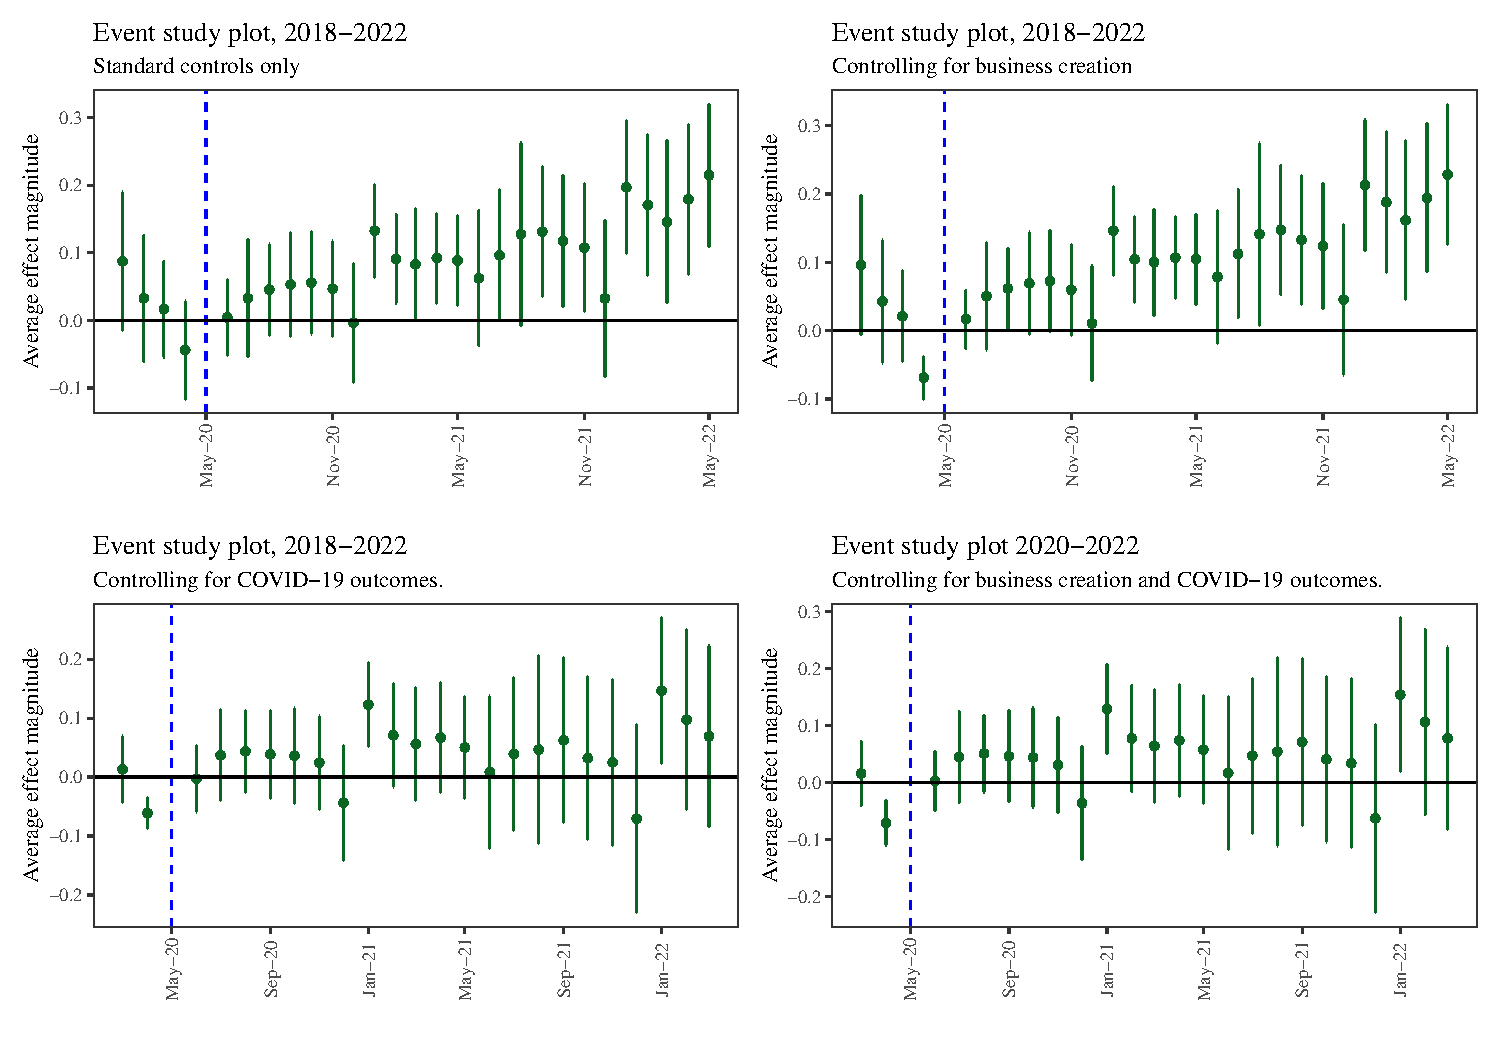
\includegraphics[width=\maxwidth]{figure/event-study1-1} 
\end{knitrout}
\end{figure}

\end{document}
